% MICAI 2026 - Springer LNCS format
\documentclass[runningheads]{llncs}

\usepackage[utf8]{inputenc}
\usepackage[T1]{fontenc}
\usepackage{graphicx}
\usepackage{booktabs}
\usepackage{amsmath,amssymb}
\usepackage{hyperref}
\usepackage{xcolor}
\usepackage{multirow}
\usepackage{array}
\usepackage{caption}
\usepackage{subcaption}

\hypersetup{colorlinks=true,linkcolor=blue,citecolor=blue,urlcolor=blue}

\begin{document}

\title{A Benchmark of Five Machine-Learning Architectures \\for Daily Trading-Signal Classification on US Tech Equities}

\titlerunning{ML Benchmark for Daily Trading Signals}

\author{Author Name\inst{1}\orcidID{0000-0000-0000-0000}}

\authorrunning{Author N.}

\institute{Institution, City, Country \\
\email{author@institution.edu}}

\maketitle

\begin{abstract}
We benchmark five supervised classifiers --- multinomial logistic regression (LR), XGBoost, a bidirectional LSTM, a 1-D CNN, and a hybrid CNN-LSTM --- on the task of predicting daily BUY/HOLD/SELL signals for seven large-cap US technology stocks (AAPL, NVDA, TSLA, AMZN, MSFT, GOOGL, META). The label is derived from the rolling 30/70-percentile of the one-day forward log-return over a 252-day window, producing an adaptive ground truth that is robust to bull/bear regimes. We use 61 indicators built from daily OHLCV plus SPY and VIX context, all obtained for free from Yahoo Finance. Three temporal splits share the same test year (2025) but differ in the number of training years (10, 6 and 4). Each architecture is trained both \emph{globally} (one model for all tickers) and \emph{per ticker}, yielding 120 controlled runs. We report F1-macro alongside three backtest metrics --- win rate, profit factor and maximum drawdown --- to capture both classification and economic quality. LR with elasticnet regularization achieves the highest average F1-macro (0.399) and the best Sharpe ratio in the principal experiment (+0.76), outperforming the deep architectures. A separate ablation shows that statistical feature filtering (Pearson, VIF, Spearman, SHAP) hurts performance in 11 of 15 cases: internal model regularization is more effective than external pre-selection. We also find that ticker volatility is the dominant factor behind cross-asset performance variation, irrespective of the model class.
\keywords{Trading signals \and Classification \and Deep learning \and Logistic regression \and XGBoost \and LSTM \and CNN.}
\end{abstract}

\section{Introduction}

Short-term forecasting of equity prices is one of the most studied problems in quantitative finance. The Efficient Market Hypothesis~\cite{fama1970} predicts that meaningful predictability should not exist; in practice, recent surveys~\cite{sezer2020,jiang2021} show that machine-learning models can extract a small but exploitable signal from technical indicators. The literature, however, suffers from three recurring limitations: (i) comparisons usually involve only one or two architectures; (ii) the reported metric is often accuracy or RMSE, which do not translate cleanly to trading performance; and (iii) feature pre-selection by univariate statistical tests is applied without checking whether it actually helps. This paper addresses these three points jointly.

We compare five representative architectures --- a linear baseline (LR), a gradient-boosted tree model (XGBoost), and three deep models (LSTM, CNN, CNN-LSTM) --- under an identical protocol across 120 controlled runs (5 models $\times$ 3 splits $\times$ 8 modalities). All runs share the same test year (2025) for a fair comparison, and only the amount of training history differs (10, 6 or 4 years). For every run we report F1-macro together with three backtest metrics: win rate, profit factor and maximum drawdown.

\paragraph{Contributions.}
\begin{enumerate}
\item A reproducible pipeline using only free Yahoo Finance data.
\item A five-architecture benchmark with 120 runs and dual evaluation (classification + economics).
\item Temporally aligned splits (same test year) that isolate the effect of training-window size.
\item An empirical assessment of statistical feature selection (Pearson, VIF, Spearman, SHAP) against using all features.
\item A discussion of why ticker volatility, rather than model choice, explains most of the cross-asset variance in Sharpe.
\end{enumerate}

\section{Related Work}
\label{sec:related}

Sezer et al.~\cite{sezer2020} review more than 140 papers on deep learning for financial time series and observe that LSTM and CNN dominate the published architectures, while linear baselines are rarely included for comparison. Fischer and Krauss~\cite{fischer2018} apply LSTM to S\&P 500 constituents and report a positive abnormal return, although later replications have raised concerns about look-ahead bias in the percentile-based label definition. Patel et al.~\cite{patel2015} compare SVM, ANN and random forest on the Indian market and find that well-regularized linear and tree models match deep networks at daily horizons. For tree-based methods, XGBoost~\cite{chen2016} remains a strong baseline; we tune it with the TPE sampler of Optuna~\cite{akiba2019}. The literature does not appear to contain a side-by-side comparison of LR, XGBoost and three different deep architectures under one experimental protocol, with both classification and economic evaluation; that is the gap addressed here.

\section{Data and Target}
\label{sec:data}

\subsection{Assets and source}

We use the seven largest US technology stocks by market capitalization at the end of 2024: AAPL, NVDA, TSLA, AMZN, MSFT, GOOGL and META. Daily OHLCV data from 2013-12-31 to 2025-12-29 are downloaded with the \texttt{yfinance} library, with adjustments for splits and dividends. Market context is added through SPY (S\&P 500 ETF) and \verb|^|VIX. No paid data source is used; the entire pipeline runs on freely available Yahoo Finance data.

\subsection{Target construction}

Let $C_t$ be the close price on day $t$. The forward log-return is
\begin{equation}
r_{\text{fwd}}(t) = \ln\frac{C_{t+1}}{C_t}.
\end{equation}
Over a rolling window of $W = 252$ trading days, we compute the 30th and 70th percentiles of $r_{\text{fwd}}$ using only data available before day $t$. The label is
\begin{equation}
y_t = \begin{cases}
\mathrm{BUY}\;(2) & \text{if } r_{\text{fwd}}(t) \ge q_{70}(t-1),\\
\mathrm{SELL}\;(0) & \text{if } r_{\text{fwd}}(t) \le q_{30}(t-1),\\
\mathrm{HOLD}\;(1) & \text{otherwise.}
\end{cases}
\end{equation}
By construction the class distribution is close to 30/40/30 in every market regime, removing the need to set an arbitrary $\alpha\sigma$ threshold. The shift by one day in the quantile computation prevents look-ahead.

\subsection{Features (61 in total)}

We compute the indicators in Table~\ref{tab:features}. All values are derived from daily OHLCV plus SPY and VIX. Seasonality variables are encoded as sine/cosine pairs to preserve periodicity. No fundamentals, news or option data are used.

\begin{table}[t]
\centering
\caption{Feature categories. All indicators are derived from OHLCV; SPY/VIX provide market context.}
\label{tab:features}
\begin{tabular}{lcl}
\toprule
Category & Count & Examples \\
\midrule
Log returns & 5 & ret\_1d, ret\_2d, ret\_3d, ret\_5d, ret\_10d \\
Momentum & 4 & mom\_5d, mom\_20d, mom\_60d \\
Moving averages & 9 & dist\_ma$\{10,20,50,200\}$, 3 crossovers, slope MA20 \\
Volatility & 8 & ATR(14), realized vol 5/10/20/60d, 2 ratios \\
Oscillators & 9 & RSI(7,14), MACD/signal/hist, Stoch K/D/diff, Williams \%R \\
Volume/flow & 8 & OBV, VWAP distance, CMF(20), MFI(14), vol\_ratio \\
Candle patterns & 7 & body/range, upper/lower shadow, gap, HL ratio \\
Seasonality & 5 & weekday and month (sine/cosine), week-of-month \\
Market context & 6 & SPY return/vol/momentum, VIX level/change/normalized \\
\midrule
\textbf{Total} & \textbf{61} & \\
\bottomrule
\end{tabular}
\end{table}

\subsection{Temporal splits}

We define three splits that share the same out-of-sample year (2025) and only differ in the amount of training history (Table~\ref{tab:splits}). This design isolates the effect of the training-window length on the comparison.

\begin{table}[t]
\centering
\caption{Temporal splits. All three share the same test year (2025) for direct comparison.}
\label{tab:splits}
\begin{tabular}{cccccc}
\toprule
Experiment & Train & Validation & Test & Train years \\
\midrule
A & 2014--2023 & 2024 & 2025 & 10 \\
B & 2018--2023 & 2024 & 2025 & 6 \\
C & 2020--2023 & 2024 & 2025 & 4 \\
\bottomrule
\end{tabular}
\end{table}

\section{Models}
\label{sec:models}

\paragraph{Logistic regression (LR).}
A multinomial logistic regressor with elasticnet penalty ($\ell_1+\ell_2$, SAGA solver). The grid over $C \in \{0.01, 0.1, 1\}$ and $l_1\text{-ratio}=0.5$ is searched on validation; class weights are balanced; multi-seed averaging combines five seeds by majority vote.

\paragraph{XGBoost.}
Gradient-boosted trees with \texttt{multi:softprob} objective and \texttt{hist} method on GPU. Hyper-parameters are tuned with Optuna~\cite{akiba2019} (TPE sampler) for 20 to 40 trials per setting, targeting validation F1-macro. Sample weights are balanced; three random seeds are averaged by soft-voting.

\paragraph{LSTM (bidirectional).}
Two stacked bidirectional LSTM layers (hidden=128, dropout=0.3) followed by layer normalization and a linear head. We evaluate look-back windows of 20 and 60 trading days. The last hidden state feeds the classifier. Three seeds are averaged.

\paragraph{1-D CNN.}
Three Conv1D blocks (filters 64-128-192, kernel=3, BN, ReLU, dropout) followed by global average $+$ max pooling along the temporal axis. Two dense layers produce the logits. No recurrence is used.

\paragraph{CNN-LSTM.}
A CNN front-end (filters 64-128) extracts local patterns; its output is fed into an LSTM (hidden=128, two layers) that captures longer dependencies. A linear head produces the logits. The last five input channels carry locally normalized OHLCV (each window divided by its first close and max volume) so that the CNN learns scale-invariant candle shapes.

\paragraph{Training and selection.}
Inputs are scaled inside each split: \texttt{StandardScaler} for LR, \texttt{MinMaxScaler} for the deep models; XGBoost takes the raw values. The deep models train for up to 80 epochs with AdamW, gradient clipping at 1.0 and \texttt{ReduceLROnPlateau} on validation loss; early stopping with patience 15 is applied. The final per-run prediction is the average of three random-seed checkpoints (five for LR).

\section{Evaluation}
\label{sec:eval}

\subsection{Classification}
We use \textbf{F1-macro} as the primary metric: the unweighted mean of the per-class F1 scores. Macro averaging gives equal weight to the BUY, HOLD and SELL classes, which is appropriate given the deliberate near-balance of the label distribution. We report per-class F1 in the appendix.

\subsection{Backtest}
For every test day the predicted label is mapped to a position: BUY $\to$ +1, HOLD $\to$ 0, SELL $\to$ -1. Daily strategy return is $r_{\text{strat}}(t) = \text{position}(t)\cdot r_{\text{fwd}}(t)$. We report:
\begin{itemize}
\item \textbf{Win rate}: fraction of trading days with $r_{\text{strat}} > 0$ among the days that the model takes a position (HOLD days excluded).
\item \textbf{Profit factor}: $\sum r_{\text{strat}}^{+} / |\sum r_{\text{strat}}^{-}|$, where the sums are over the same set of days.
\item \textbf{Maximum drawdown}: minimum of $(\text{equity}_t - \text{peak}_t)/\text{peak}_t$ on the cumulative equity curve.
\item \textbf{Annualized Sharpe ratio}: $\sqrt{252}\;\bar r_{\text{strat}}/\sigma_{r_{\text{strat}}}$, with $r_f = 0$.
\end{itemize}
We deliberately omit transaction costs and slippage; the assumption is a first-order comparison between models under identical conditions.

\subsection{A note on accuracy}
We do not report accuracy. With three near-equally-distributed classes, the classifier can reach $\approx$~0.40 accuracy by predicting only HOLD, which is uninformative. F1-macro penalizes such collapse.

\section{Statistical feature pre-selection: should we use it?}
\label{sec:featselect}

A common preliminary step is to filter features through statistical tests: Pearson correlation against the target, VIF for multicollinearity (suited to LR), SHAP rank (suited to tree models), or Spearman rank correlation (more appropriate for the non-linear models). We compared, on the same code path, every model trained with the full 61 features against the same model trained with only those features that passed its corresponding test on the validation set.

\begin{table}[t]
\centering
\caption{Effect of statistical pre-selection on GLOBAL F1-macro: $\Delta = \text{F1}(\text{all 61}) - \text{F1}(\text{filtered})$. A positive value means that using all features is better.}
\label{tab:featselect}
\begin{tabular}{lccc}
\toprule
Model & Filter & Exp A & Exp B & Exp C \\
\midrule
LR & Pearson + VIF (4--8 feats)& $+0.024$ & $+0.026$ & $+0.021$ \\
XGBoost & SHAP top-$N$ (23--25 feats)& $+0.009$ & $+0.021$ & $+0.022$ \\
LSTM & Spearman (3--25 feats)& $+0.039$ & $+0.036$ & $-0.006$ \\
CNN-1D & Spearman & $+0.035$ & $-0.025$ & $+0.011$ \\
CNN-LSTM & Spearman & $-0.011$ & $+0.020$ & $-0.026$ \\
\bottomrule
\end{tabular}
\end{table}

\paragraph{Result.}
Table~\ref{tab:featselect} shows that in 11 of 15 cases keeping all 61 features beats the filtered subset. The deltas are largest for LR (the model with the strongest internal regularization), where the elasticnet penalty performs implicit selection more effectively than the external Pearson/VIF screen. For XGBoost the SHAP-based filter is competitive (smallest deltas), as expected for a tree model. For the deep models the result depends on the experiment.

\paragraph{Decision.}
All subsequent results use the full 61 features for every model. The Pearson/VIF/Spearman/SHAP tests are still useful as exploratory tools (e.g.\ to communicate which indicators dominate), but they should not be used as a pre-training filter.

\section{Results}
\label{sec:results}

We report 120 controlled runs (5 models $\times$ 3 splits $\times$ (1 global + 7 per-ticker)). Throughout this section ``best lookback'' is selected on the validation set when applicable (LSTM, CNN, CNN-LSTM).

\subsection{Global models}

Table~\ref{tab:f1_global} shows F1-macro on the 2025 test set when one single model is trained on the concatenated data of all seven tickers. LR leads on average (0.399) and wins two of the three experiments outright. XGBoost is the runner-up and edges LR by one point in Exp B. The deep models cluster lower, around 0.34--0.39.

\begin{table}[t]
\centering
\caption{F1-macro on the 2025 test set, GLOBAL strategy. Best per column in bold.}
\label{tab:f1_global}
\begin{tabular}{lcccc}
\toprule
Model & Exp A (10y) & Exp B (6y) & Exp C (4y) & Avg \\
\midrule
LR & \textbf{0.411} & 0.385 & \textbf{0.401} & \textbf{0.399} \\
XGBoost & 0.396 & \textbf{0.386} & 0.373 & 0.385 \\
LSTM & 0.389 & 0.370 & 0.370 & 0.376 \\
CNN-LSTM & 0.376 & 0.384 & 0.371 & 0.377 \\
CNN 1D & 0.361 & 0.343 & 0.373 & 0.359 \\
\midrule
Random 1/3 & 0.333 & 0.333 & 0.333 & 0.333 \\
\bottomrule
\end{tabular}
\end{table}

\begin{figure}[t]
\centering
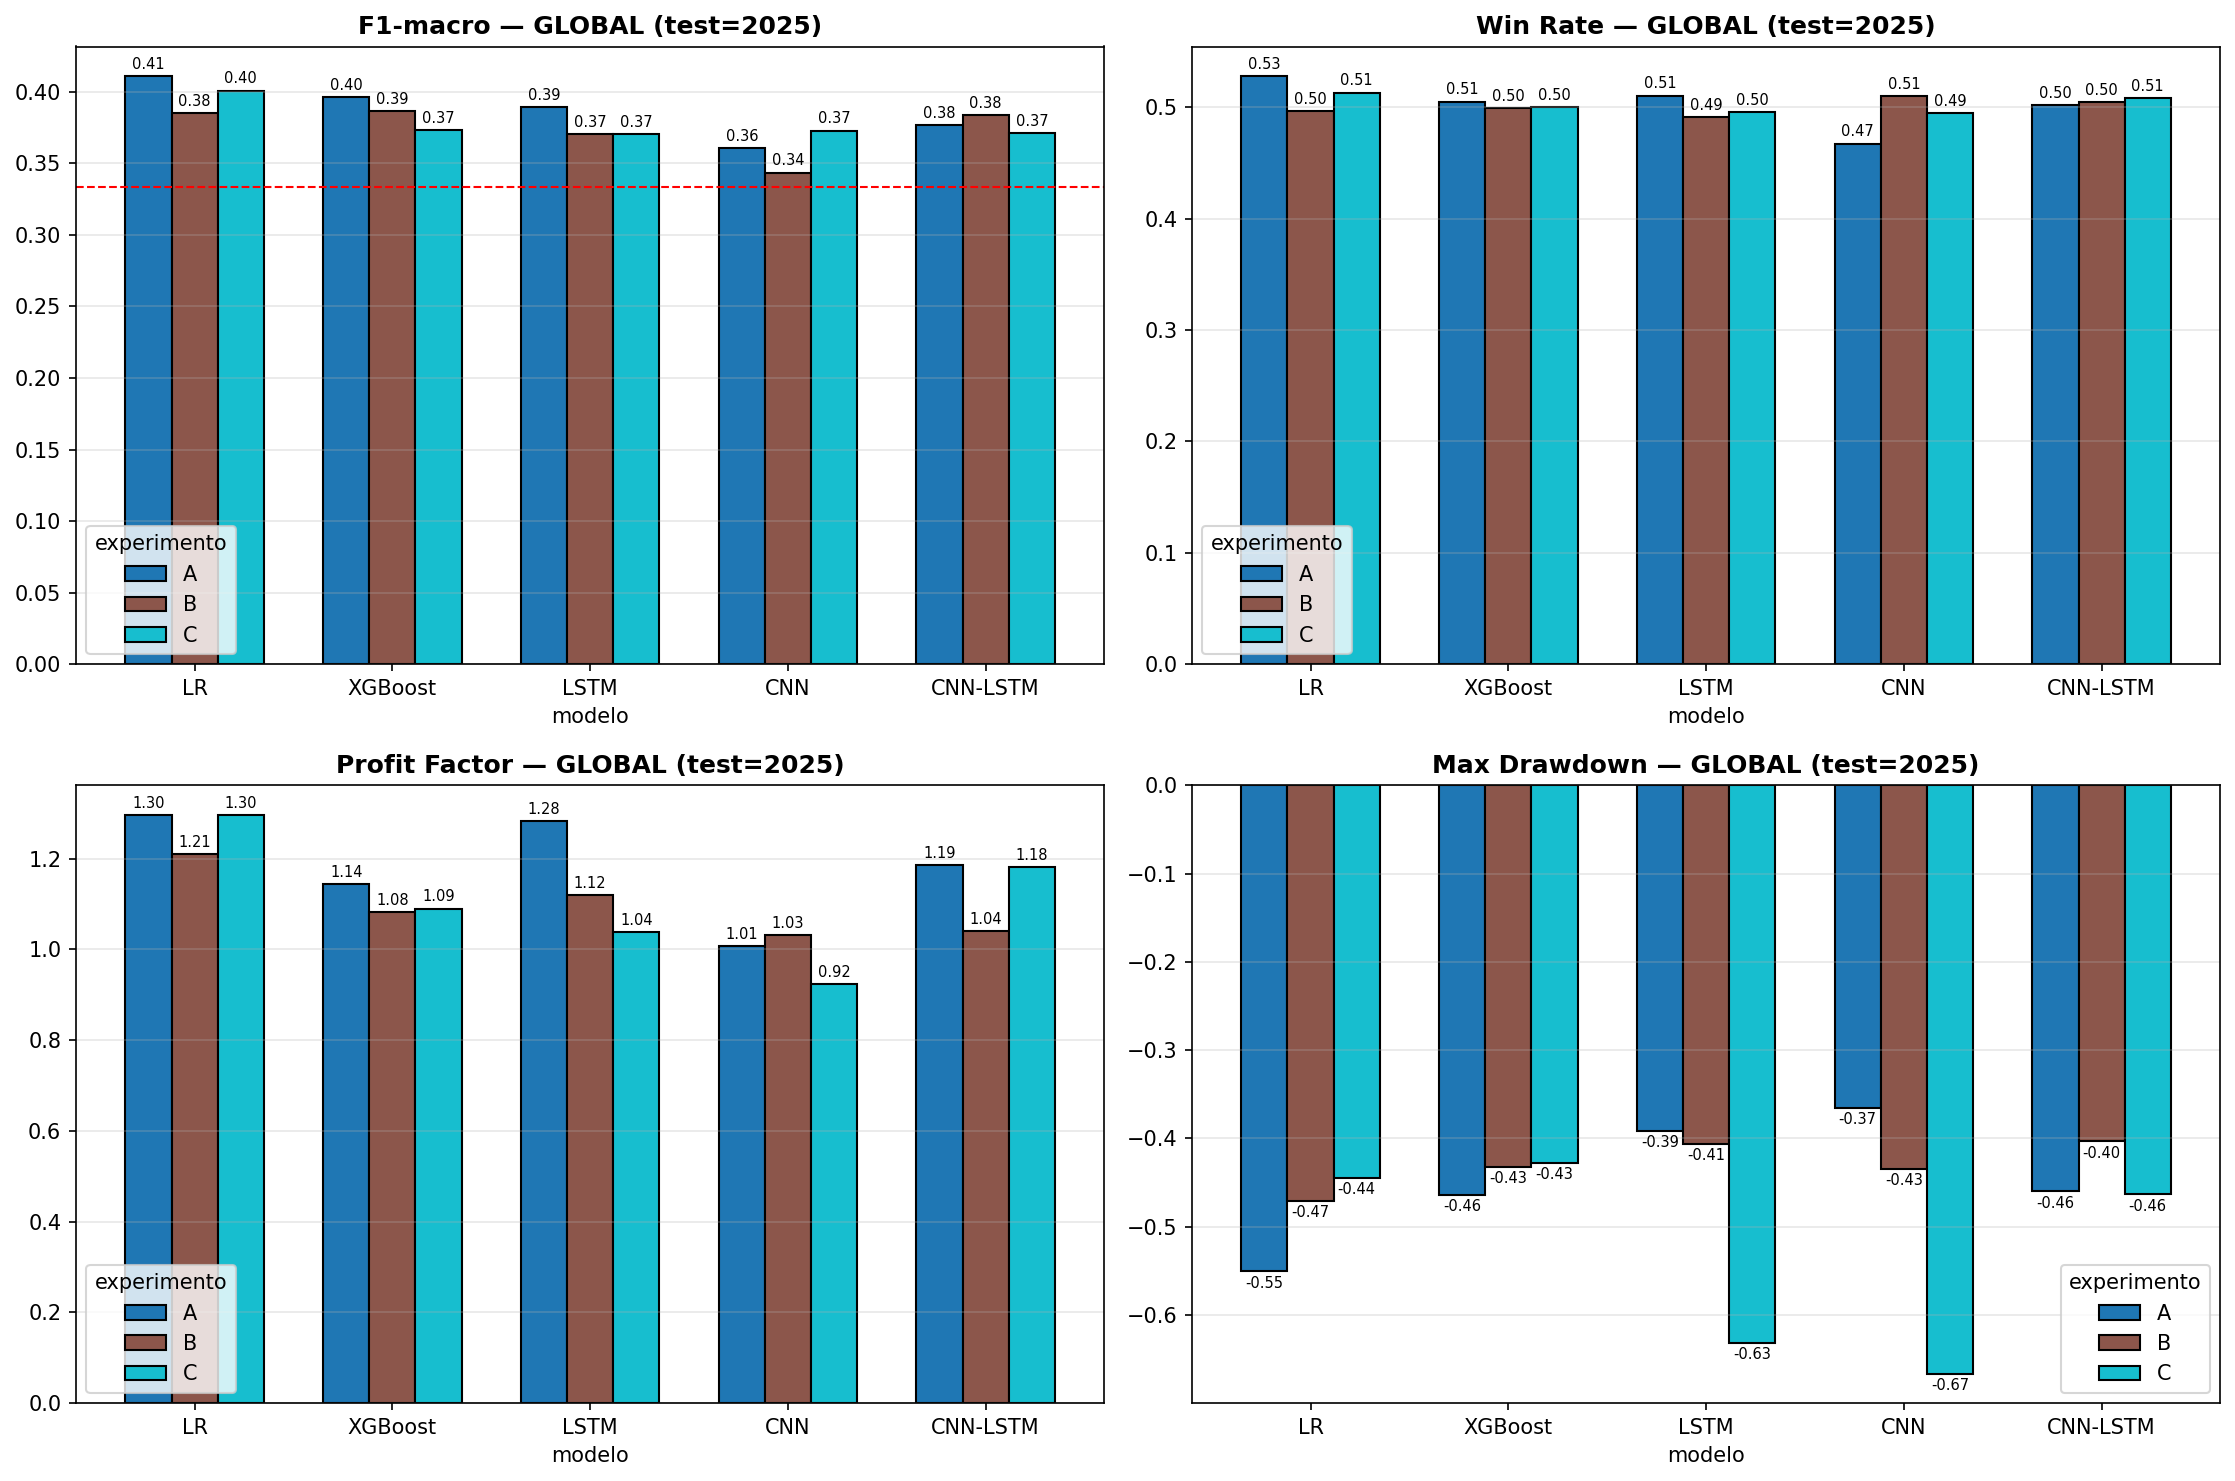
\includegraphics[width=\textwidth]{figures/fig_global_metrics.png}
\caption{Global models on the 2025 test set: F1-macro (top-left), win rate (top-right), profit factor (bottom-left) and maximum drawdown (bottom-right). The dashed red line in the F1 panel marks the 1/3 random baseline. Higher is better except for drawdown.}
\label{fig:global}
\end{figure}

The economic metrics tell a more nuanced story (Fig.~\ref{fig:global} and Table~\ref{tab:econ_B}). For the recommended experiment (Exp B), LR has the highest profit factor (1.21) and Sharpe (+0.76). XGBoost matches the F1 but its strategy is closer to random in economic terms. CNN-LSTM controls drawdown best ($-0.40$). The pure CNN is the weakest both in F1 and Sharpe.

\begin{table}[t]
\centering
\caption{Economic metrics on Exp B GLOBAL (test = 2025). Sharpe is annualized.}
\label{tab:econ_B}
\begin{tabular}{lccccc}
\toprule
Model & F1 & Win rate & Profit factor & Max drawdown & Sharpe \\
\midrule
LR & 0.385 & 0.497 & \textbf{1.210} & $-0.470$ & \textbf{+0.755} \\
XGBoost & \textbf{0.386} & 0.500 & 1.083 & $-0.432$ & +0.345 \\
CNN-LSTM & 0.384 & \textbf{0.505} & 1.041 & \textbf{$-$0.403} & +0.147 \\
LSTM & 0.370 & 0.491 & 1.120 & $-0.406$ & +0.433 \\
CNN 1D & 0.343 & 0.510 & 1.031 & $-0.434$ & +0.121 \\
\bottomrule
\end{tabular}
\end{table}

\subsection{Per-ticker models}

When one model is trained per ticker (Table~\ref{tab:f1_pt}), LR is again the most consistent: it leads in all three experiments. The deep models drop more visibly compared to the global setting, because each per-ticker training set contains only $\sim$1500 samples. XGBoost remains a solid second.

\begin{table}[t]
\centering
\caption{Average F1-macro across 7 tickers, PER-TICKER strategy. Best per column in bold.}
\label{tab:f1_pt}
\begin{tabular}{lcccc}
\toprule
Model & Exp A & Exp B & Exp C & Avg \\
\midrule
LR & \textbf{0.411} & \textbf{0.392} & \textbf{0.359} & \textbf{0.387} \\
XGBoost & 0.376 & 0.370 & 0.352 & 0.366 \\
CNN-LSTM & 0.368 & 0.342 & 0.356 & 0.355 \\
LSTM & 0.314 & 0.353 & 0.326 & 0.331 \\
CNN 1D & 0.378 & 0.332 & 0.280 & 0.330 \\
\bottomrule
\end{tabular}
\end{table}

\subsection{Where does the cross-asset variation come from?}

Figure~\ref{fig:sharpe_heatmap} breaks down the annualized Sharpe by model and ticker. Vertical bands are visible: AMZN and TSLA tend to be green across models, while GOOGL is red. This is a property of the assets, not of the models: the more directionally tradeable tickers (high realized vol, well-defined trends) reward any reasonable classifier, while range-bound tickers punish all of them. Averaging the per-model standard deviation across tickers (0.62 to 0.93) shows that the model contributes substantially less than the ticker to the total Sharpe variance.

\begin{figure}[t]
\centering

\includegraphics[width=\textwidth]{figures/fig_sharpe_heatmap.png}
\caption{Annualized Sharpe ratio per model and ticker, for the three experiments (test = 2025).}
\label{fig:sharpe_heatmap}
\end{figure}

\begin{figure}[t]
\centering

\includegraphics[width=0.85\textwidth]{figures/fig_sharpe_boxplot.png}
\caption{Sharpe distribution per ticker over the 15 (model, experiment) combinations. Diamonds mark the mean. AMZN dominates; GOOGL is the only ticker with a negative median.}
\label{fig:sharpe_box}
\end{figure}

\subsection{Effect of the training-window length}

The three splits share the same test year, so any difference between them is purely the effect of how many years of history the model can fit. Figure~\ref{fig:trainyears} suggests that LR benefits monotonically from longer histories (Exp A: 0.411 $>$ Exp B: 0.385 $>$ Exp C: 0.401, with a small Exp C rebound). The deep models are largely flat, indicating that more history does not help much when capacity is fixed and the optimizer is the bottleneck.

\begin{figure}[t]
\centering

\includegraphics[width=\textwidth]{figures/fig_train_years.png}
\caption{Effect of training-window length on F1-macro (left) and Sharpe (right). All settings test on year 2025.}
\label{fig:trainyears}
\end{figure}

\subsection{Signal distribution}

Figure~\ref{fig:signaldist} shows the predicted distribution of BUY/HOLD/SELL labels for the five global models on Exp B. The base rate is roughly 30/40/30. CNN 1D collapses heavily towards BUY (49\,\%); LR is the most balanced but slightly conservative on BUY (18\,\%). This asymmetry is a useful diagnostic: a model whose predicted distribution is far from the prior is either over-confident on one side or has converged to a degenerate solution.

\begin{figure}[t]
\centering

\includegraphics[width=0.95\textwidth]{figures/fig_signal_dist.png}
\caption{Predicted distribution of the three signals for the global models on Exp B (test=2025). Dotted lines indicate the 33.3\,\% / 66.6\,\% references.}
\label{fig:signaldist}
\end{figure}

\subsection{Drill-down on the best model per ticker}

Table~\ref{tab:tsla_drill} reports the per-ticker breakdown of the highest F1 model in Exp B (XGBoost). TSLA is the outlier: F1 $=$ 0.44, Sharpe $=$ +2.06, +201\,\% cumulative return. The lowest performer is GOOGL with negative Sharpe.

\begin{table}[t]
\centering
\caption{Per-ticker drill-down for XGBoost Exp B GLOBAL (test = 2025).}
\label{tab:tsla_drill}
\begin{tabular}{lccccc}
\toprule
Ticker & F1-macro & Sharpe & Cum.\ return & Win rate & Max DD \\
\midrule
\textbf{TSLA} & \textbf{0.441} & \textbf{+2.06} & \textbf{+2.01} & 0.604 & $-0.20$ \\
MSFT & 0.399 & $-0.06$ & $-0.01$ & 0.473 & $-0.22$ \\
AMZN & 0.390 & +0.57 & +0.19 & 0.531 & $-0.21$ \\
META & 0.347 & +0.71 & +0.27 & 0.470 & $-0.18$ \\
NVDA & 0.338 & +1.41 & +0.77 & 0.539 & $-0.37$ \\
AAPL & 0.336 & +0.27 & +0.08 & 0.513 & $-0.24$ \\
GOOGL & 0.336 & $-0.88$ & $-0.21$ & 0.487 & $-0.35$ \\
\bottomrule
\end{tabular}
\end{table}

\section{Discussion}
\label{sec:discussion}

\paragraph{Why does LR win on F1?}
With approximately 1500 training samples per ticker (10\,500 globally) and 61 inputs, deep models with $10^5$--$10^6$ parameters are firmly in an overfitting regime. The technical indicators already capture most of the linear predictive content of price action; the elasticnet penalty selects an effective subset of them automatically and stabilizes the remaining coefficients. XGBoost shows similar resilience because tree pruning and the L2 leaf penalty play the same role.

\paragraph{Why is the cross-asset variation so large?}
Section~6.3 indicates that the model accounts for a smaller share of Sharpe variance than the ticker does. Tickers with persistent trends or high realized volatility (AMZN, TSLA, NVDA) reward any reasonably calibrated classifier; range-bound tickers (GOOGL) do not. This has practical consequences: a portfolio constructor would do better to pre-screen tickers by predictability than to choose a more elaborate model class.

\paragraph{Global vs.\ per ticker.}
Aggregating tickers into one global training set helps LR and XGBoost (Tables \ref{tab:f1_global} and \ref{tab:f1_pt}: 0.411 vs.\ 0.354 in Exp A, 0.385 vs.\ 0.392 in Exp B). The deep models do not benefit as much, presumably because the inter-ticker pattern they extract from the larger dataset is close to what each per-ticker model already finds.

\paragraph{When should one use the deep models?}
LSTM and CNN-LSTM produce competitive economic metrics on the volatile tickers, sometimes with smaller drawdown than LR. They become attractive when (i)~the application requires modeling temporal dependencies beyond the look-back of the features themselves and (ii)~enough training history is available to justify the parameter count. In our setting, neither condition is decisively met.

\section{Limitations}
\label{sec:limitations}

We do not include transaction costs or slippage; under realistic costs the rank order between models with $\text{Sharpe}\!<\!0.5$ would likely flip in favor of the strategy that trades least. The sample is restricted to seven large-cap US technology stocks, so the conclusions need not generalize to other sectors or markets. Position sizing is binary ($\pm 1$ or $0$); a Kelly or volatility-targeted scheme would change the absolute Sharpe figures while keeping the relative ranking. We use a single train/validation/test split per experiment; a walk-forward protocol with multiple folds would tighten the confidence intervals at significantly higher compute cost.

\section{Conclusions}
\label{sec:conclusions}

A multinomial logistic regression with elasticnet regularization, trained on 61 indicator features derived from free Yahoo Finance data, beats three different deep architectures and a tuned XGBoost on average F1-macro across three temporal splits, and matches or exceeds them on the economic metrics. Statistical feature pre-selection (Pearson, VIF, Spearman, SHAP) does not help: keeping all features and relying on the model's own regularization wins in 11 out of 15 cases. Ticker volatility, not model class, explains the bulk of the cross-asset Sharpe variation. For practitioners working with daily large-cap data and no access to alternative datasets, a well-regularized linear classifier is a competitive and computationally cheap default; deep models become attractive only with longer histories or richer inputs.

\paragraph{Reproducibility.}
All code and data manifests are available in the supplementary material. Random seeds are fixed and listed per run; library versions match those in \texttt{requirements.txt}.

\begin{thebibliography}{9}

\bibitem{fama1970}
Fama, E. F.: Efficient capital markets: A review of theory and empirical work. The Journal of Finance \textbf{25}(2), 383--417 (1970)

\bibitem{sezer2020}
Sezer, O. B., Gudelek, M. U., Ozbayoglu, A. M.: Financial time series forecasting with deep learning: A systematic literature review. Applied Soft Computing \textbf{90}, 106181 (2020)

\bibitem{fischer2018}
Fischer, T., Krauss, C.: Deep learning with long short-term memory networks for financial market predictions. European Journal of Operational Research \textbf{270}(2), 654--669 (2018)

\bibitem{jiang2021}
Jiang, W.: Applications of deep learning in stock market prediction: recent progress. Expert Systems with Applications \textbf{184}, 115537 (2021)

\bibitem{patel2015}
Patel, J., Shah, S., Thakkar, P., Kotecha, K.: Predicting stock and stock price index movement using trend deterministic data preparation and machine learning techniques. Expert Systems with Applications \textbf{42}(1), 259--268 (2015)

\bibitem{chen2016}
Chen, T., Guestrin, C.: XGBoost: A scalable tree boosting system. In: Proc. KDD, pp. 785--794. ACM (2016)

\bibitem{akiba2019}
Akiba, T., Sano, S., Yanase, T., Ohta, T., Koyama, M.: Optuna: A next-generation hyperparameter optimization framework. In: Proc. KDD, pp. 2623--2631 (2019)

\bibitem{hochreiter1997}
Hochreiter, S., Schmidhuber, J.: Long short-term memory. Neural Computation \textbf{9}(8), 1735--1780 (1997)

\bibitem{lecun1989}
LeCun, Y., Boser, B., Denker, J. S., et al.: Backpropagation applied to handwritten zip code recognition. Neural Computation \textbf{1}(4), 541--551 (1989)

\bibitem{lundberg2017}
Lundberg, S. M., Lee, S.-I.: A unified approach to interpreting model predictions. In: Advances in Neural Information Processing Systems, pp. 4765--4774 (2017)

\bibitem{zou2005}
Zou, H., Hastie, T.: Regularization and variable selection via the elastic net. Journal of the Royal Statistical Society B \textbf{67}(2), 301--320 (2005)

\bibitem{lopezdeprado2018}
L\'opez de Prado, M.: Advances in Financial Machine Learning. Wiley (2018)

\end{thebibliography}

\end{document}
